\section{Морфологическая обработка данных и анализ текста}

В данной секции в качестве входа используются файлы, полученные после запуска экстрактора, описанного в предыдущений секции. В целях сохранения независимости этапов обработки, а также избежание повторного запуска экстрактора была написана отдельная утилита \href{https://github.com/vasalf/hse-web-search-homework/blob/master/1/apply.py}{apply.py}, осуществляющая обработку текста, очищенного от html-тэгов и подсчёт статистик. 

\paragraph{Архитектура}

Для более эффективного использования ресурсов, гибкости разработки и минимализации конфликтов между разработчиками был реализован \href{https://refactoring.guru/ru/design-patterns/chain-of-responsibility}{паттерн проектирования pipeline}. Утилита послеовательно принимает на вход файлы и пропускает их через пайплайн, состоящий из необходимого нам набора обработчиков, которые, благодаря шаблону, могут разрабатываться независимо, просто наследуясь от интерфейса обработчика. Набор и последовательность обработчиков при необходимости можно легко изменить в зависимости от наших потребностей.

Для решения текущей задачи был реализован следующий набор обработчиков (в порядке запуска):

\begin{enumerate}
	\item TextProcessorStage -- преобразует текст в набор лемматизированных слов
	\item JsonUnpackerStage -- распаковывает JSON в текстовом представлении в настоящий JSON
	\item GraphBuilder -- собирает метаданные о ссылочных рёбрах из JSONа, распакованного предыдущим обработчиком
	\item StopwordsCounter -- подсчитывает слова из лемматизированного текста, классифицируемые как стоп-слова 
	\item DictionaryStats -- собирает словари слов, ведёт на их основе подсчёт tf-idf
	\item SimpleStats -- собирает простую статистику, не требующую хранения данных или использования внешних библиотек (например, среднюю длину слов).	
\end{enumerate}

После того, как какждый документ был обработан пайплайном, у каждого обработчика вызывается метод dump, обрабатывающий полученные результаты, после чего происодит вывод на экран/запись результатов в файл/рендеринг графика и т.д. 

В случае необходимости такую архитектуру можно легко распараллелить по данным, создав несколько экземпляров пайплайна и распределив между ними файлы. 

Для большей наглядности ниже приведена диграмма классов: 

\begin{figure}
	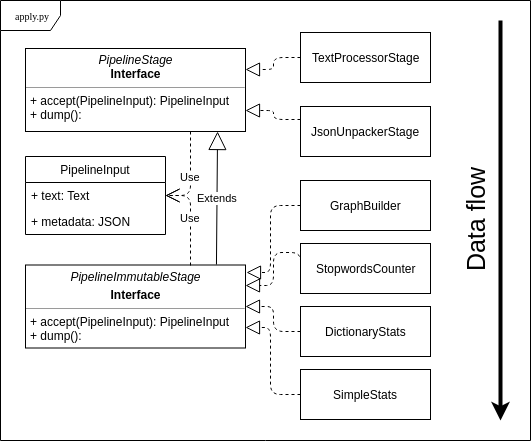
\includegraphics[width=.5\textwidth]{apply_uml_data_flow.png}
	\caption{UML-диаграмма классов пайплайна}
	\label{apply-uml}
\end{figure}

Классы, унаследованные от \texttt{PipelineImmutableStage} гаранитированно пропустят через себя \texttt{PipelineInput} без изменений. Это сделано, чтобы дополнительно обезопасить себя от ошибок.


\paragraph{Обработка текста}

Полученный от экстрактора файл конкатенировался в одну строку, переводился в нижний регистр, после чего токенизировался и леммматизировался с помощью библиотеки \texttt{mystem} методом \texttt{Mystem.lemmatize}. После этого полученный набор токенов фильтровался на предмет принадлежности множеству слов на одном из трёх языков: русском, беларусском или английском. 

Здесь и далее определение языка слова происходит следующим образом:

Токен считается:
\begin{itemize}
	\item Словом на английском языке, если он состоит исключительно из букв набора ''abcdefghijklmnopqrstuvwxyzéôïç'' (некоторые слова английского языка имеют французское происхождение).
	
	\item Словом на русском языке, если он состоит исключительно из букв набора ''абвгдеёжзийклмнопрстуфхцчшщьыъэюя''
	
	\item Словом на белорусском языке, если он состоит исключительно из букв набора ''абвгдеёжзiйклмнопрстуўфхцчшьыэюя''
\end{itemize}

Сразу стоит оговориться, что для некоторых слов мы не можем сказать, на русском или белорусском языке оно написано ввиду большого пересечения алфавитов, поэтому многие из последующих статистик посчитаны для русских и балорусских слов вместе.

Также стоит заметить, что и белорусский, и русский алфавиты содержат в себе буквы, которые отсутствуют в другом языке (например, в русском нет буквы 'ў', а в белорусском 'и'), поэтому слова, состоящие из букв объединения алфавитов, но не принадлежащие ни одному алфавиту по отдельности, были отфильтрованы такой проверкой, хотя и могли иметь смысл . Тем не менее, таких слов пренебрежимо мало и их можно опустить.


\paragraph{Подсчёт статистик}

\subparagraph{Стоп-слова.}

В качестве словаря стоп-слов был использован русский и английский корпуса \texttt{stopwords} библиотеки \texttt{nltk}. Получилось, что $\sim24\%$ русских слов (29525733 из 122180991) являются стоп-словами, в то время как для английского языка это число всего лишь $\sim10\%$ (2580672 из 26412145) от слов на английском языке ($\sim11\%$, 2580672 из 23417440, если отфильтровать часто встречающиеся''ссылочные'' слова: http, url, www, com). Всего $\sim 21.6\%$ слов из документов являются стоп-словами. 

Учитывая датасет, не стоит из этого делать вывод, что в английском меньше стоп-слов. Просто в русскоязычной переписке, которой тут большинство, люди часто употребляли названия брендов/операционных стстем и утилит/может чего ещё на английском языке, которые часто пусть и односложные, но зато стоп-словами не являются (например, смотри таблицу \ref{table_english_words}). Часто то, что программа посчитала английским словом -- это кусочек url, которое может быть как частоупотребимым http, так и случайной строкой, которая была id страницы.

\subparagraph{Длины слов.}

Средняя длина русских/беларусских слов в тексте составляет $\sim 6$ символов.

Средняя длина английских слов в тексте составляет $\sim 4.8$ символов.

Без привязки к языку: $\sim 5.7$ символов.


\subparagraph{Доля английского языка} в тексте составляет $\sim 17.7\%$ (26412145 из 148775198).

\subparagraph{Частота встречаемости слов}

По мере обработки файлов накапливался словарь, в котором для каждого слова из корпуса документов было подсчитано количество его вхождений в корпус (в частности, если слово встречалось в одном документе $x$ раз, этот документ добавит этому слову $x$ раз в подсчёт частоты встречаемости). Ниже приведены топы слов по частоте встречаемости с разными фильтрами: 

\begin{table}
	\begin{center}
		\begin{tabular}{|l|c|}
			\hline
			Слово & Количество вхождений\\
			\hline
			и & 3528123 \\
			в &3357592\\
			на &1829399\\
			с &1444609\\
			не &1234956\\
			http& 1099771\\
			url &956971\\
			по &879989\\
			для& 879941\\
			быть& 770399\\
			что &712013\\
			а &690562\\
			я &646000\\
			a &617208\\
			www &608415\\
			сообщение &591339\\
			к &556471\\
			о &493412\\
			от& 479708\\
			весь& 457124\\
			\hline
		\end{tabular}
	\end{center}
	\caption{Топ-20 всех слов по частоте встречаемости.}
	\label{table_all_words_frequency}
\end{table}

На таблице \ref{table_all_words_frequency}, довольно ожидаемо, стоп-слова вырвались вперёд. Отфильтруем их.
Для большего понимания происходящего отдельно соберём топы русских и английских слов (см таблицы \ref{table_russian_words} и \ref{table_english_words}). По русскому топу можно предположить, что в 2007 году большая часть белорусских сайтов была форумами, часто новостными. Английский топ тоже показывает интересный результат. Так, например, видно, что люди часто обсуждали телефоны и порно. 

\begin{table}
	\begin{center}
		\begin{tabular}{|l|c|}
			\hline
			Слово & Количество вхождений\\
			\hline
			сообщение& 591339 \\
			весь &457124 \\
			г &449458\\
			год& 433355\\
			беларусь &355728\\
			мочь &328606\\
			новость& 302549\\
			форум &301805\\
			сайт &298328\\
			добавлять &282209\\
			работа &280959\\
			минск &280601\\
			новый &265558\\
			день &257852\\
			если &220779\\
			один &210315\\
			автор &210032\\
			пользователь &200908\\
			только &197521\\
			\hline
		\end{tabular}
	\end{center}
	\caption{Топ-20 русских сллов без стоп-слов}
	\label{table_russian_words}
\end{table}

\begin{table}
	\begin{center}
		\begin{tabular}{|l|c|}
			\hline
			Слово & Количество вхождений\\
			\hline
			nokia & 120987\\
			dvd & 119349\\
			mail & 105002\\
			free & 85601\\
			cd & 74805\\
			blowjob & 73488\\
			online & 70859\\
			samsung & 70138\\
			viagra & 63272\\
			sex & 59877\\
			cgi & 56620\\
			pm & 56412\\
			siemens & 54440\\
			sony & 51479\\
			porn & 47614\\
			web & 45874\\
			cialis & 45425\\
			cheap & 42812\\
			club & 40917\\
			video & 38942\\
			\hline
		\end{tabular}
	\end{center}
	\caption{Топ-20 английских слов без артефактов от ссылок и стоп-слов}
	\label{table_english_words}
\end{table}


\begin{table}
	\begin{center}
		\begin{tabular}{|l|c|}
			\hline
			Слово & Количество вхождений\\
			\hline
			сообщение &859336.0170794941\\
			buy &698103.6336946577\\
			blowjob &521330.10798397573\\
			г &466166.0979451989\\
			info &435700.68235274975\\
			nokia &396222.4091821661\\
			viagra &374574.95699222025\\
			руб &369364.30124008877\\
			год &360519.5542405188\\
			добавлять &338088.4421394479\\
			мочь &329356.68234718597\\
			автор &326042.95371074876\\
			беларусь &319595.3752265926\\
			зарегистрировать &317149.14969954256\\
			cgi &314349.7174971446\\
			free &311139.9577668955\\
			заголовок &294323.4515316789\\
			porn &286142.45224346535\\
			республика &282033.1417976597\\
			день &280699.6220832565\\
			\hline
		\end{tabular}
	\end{center}
	\caption{Топ-20 слов по произведению tf-idf}
	\label{table_tf_idf_top}
\end{table}

\subparagraph{Обратная частота встречаемости.}
	Для каждого слова было посчитано idf $ = \log \frac{N}{d}$, где $N$ -- количество документов всего, а $d$ -- количество документов, в которых встречается заданное слово. После этого для каждого слова было посчитано произведение частоты встречаемости в корпусе на обратную частоту. Топ слов по этому произведению можно видеть в таблице \ref{table_tf_idf_top}. 

\subparagraph{Ранк слова - частота слова.}

Также был посчитан график зависимости логарифма частоты встречаемости слова в корпусе от ранга слова. См. изображение \ref{fig_rank_to_frequency}. 

На графике видно, что чуть больше половины слов встречаются всего один-два раза. При взгляде на данные оказывается, что это специфичные словоформы (онлайниться, мужичишко, протрындеть), слова с опечатками(поттверждение, катяться, тепероь, ипрессионизм), слова на белорусском(перайдуць, ваколiцам, масаў), случайные английские строки(возможно, куски ссылок: jxnoxzhpmkiugnjyp, gwvdvstqsoeycamln), логины людей (?), редкоупотребляемые/искаженные термины (caleidochrome, frontex, debiangnulinux).


\begin{figure}
	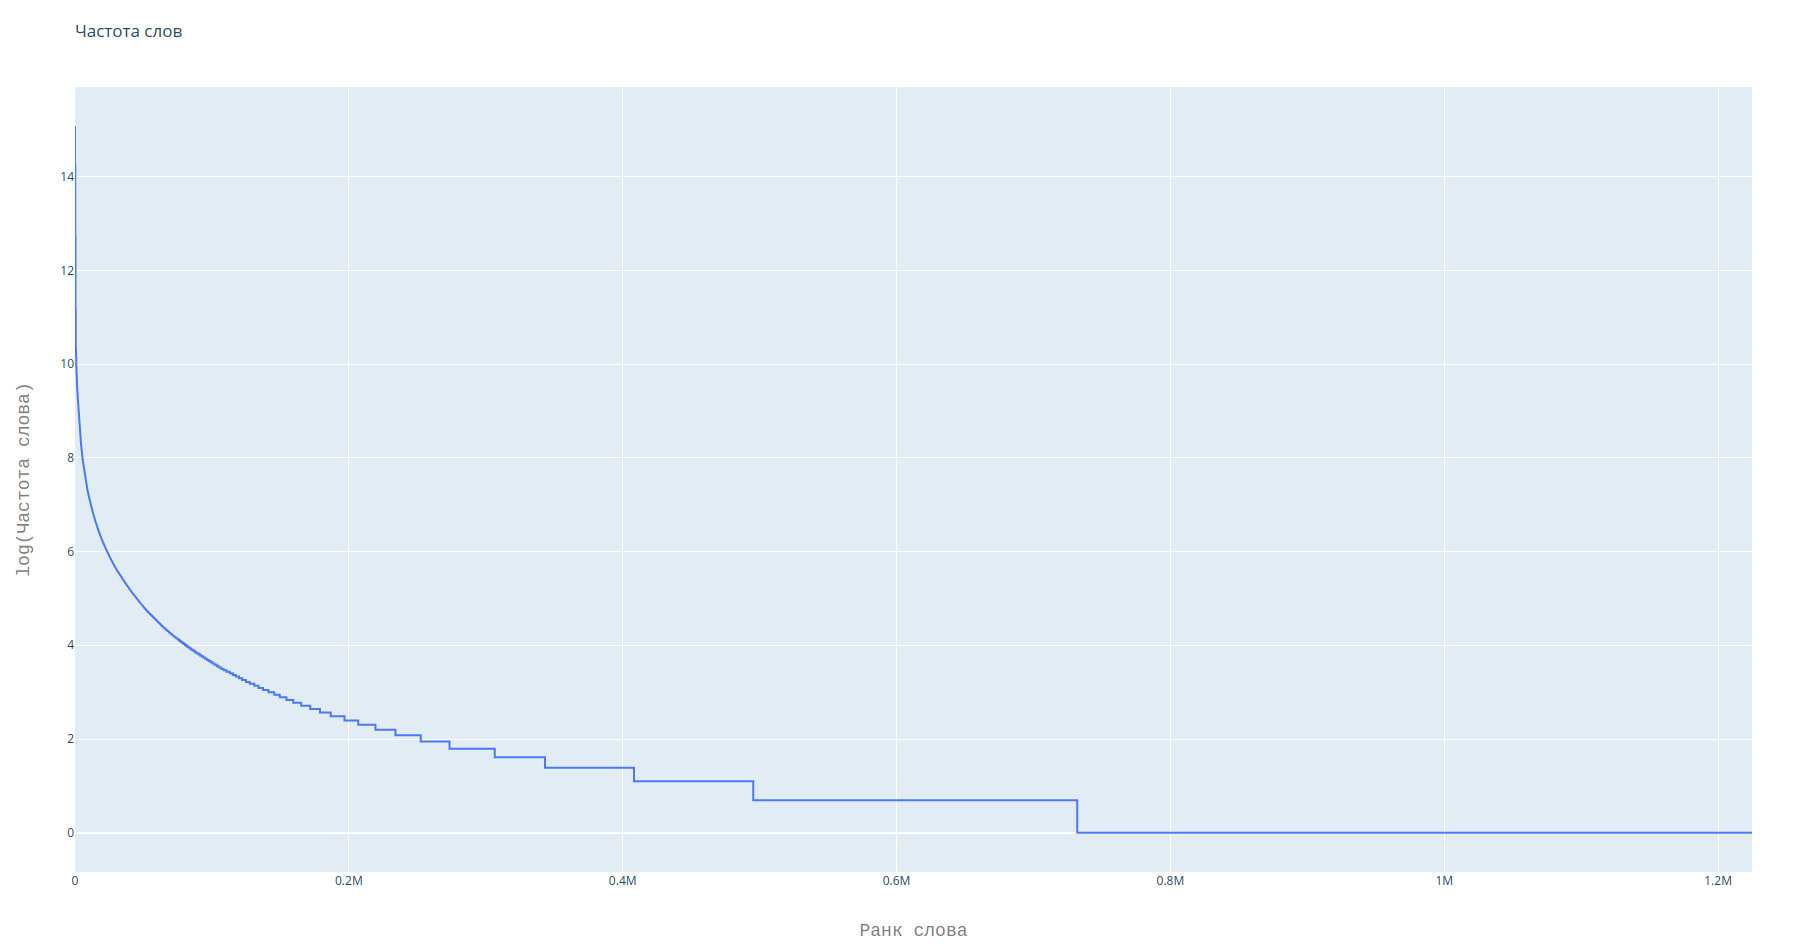
\includegraphics[width=.5\textwidth]{rank_to_frequency.png}
	\caption{Зависимость логарифма частоты встречаемости слова от его ранка.}
	\label{fig_rank_to_frequency}
\end{figure}
